\documentclass[compress]{beamer}

\usepackage[utf8]{vntex}
\usepackage{longtable,booktabs}
\usepackage{amsmath}
\usepackage{amsfonts}
\usepackage{cases}
\usepackage{amssymb}
\usepackage[utf8]{inputenc}
\usepackage[absolute,overlay]{textpos}
\usepackage{listings}
\usepackage{subcaption}
\usepackage{tikz}
\usepackage{pgfplots}
\usepackage{fancybox}
\usepackage{multirow}
\usepackage{tikz-uml}
\tikzumlset{font=\tiny}
\usepackage{multimedia}
\usetikzlibrary{arrows.meta}
\usetikzlibrary{shapes.geometric}
\PassOptionsToPackage{hyphens}{url}\usepackage{hyperref}  
\lstset{
	language = Java,
	frame = single,
	tabsize = 3
}

\usetheme{Warsaw}
%\usetheme{Antibes}
%\usecolortheme{spruce}
%\setbeamercolor{structure}{fg=cyan!90!blue}
%\newtheorem{theorem}{Định lý}[]

\expandafter\def\expandafter\insertshorttitle\expandafter{%
    \insertshorttitle\hfill%
    \insertframenumber\,/\,\inserttotalframenumber}
      
\AtBeginSection[] % Do nothing for \section*
{
\begin{frame}
\tableofcontents[currentsection]
\end{frame}
}
\AtBeginSubsection[] % Do nothing for \section*
{
\begin{frame}
\tableofcontents[currentsection, currentsubsection]
\end{frame}
}

\title[Mật mã trên đường cong Elliptic Curves cho thiết bị IoT]{Mật mã trên đường cong Elliptic Curves cho thiết bị IoT} 

\author[Đặng Quang Trung]{
Sinh viên thực hiện\\
Đặng Quang Trung - 20134145 \\[1em]
Giảng viên hướng dẫn\\
TS Trần Vĩnh Đức}
\begin{document}

\begin{frame}[plain]
\titlepage
\end{frame}

\begin{frame}[plain]{Nội dung trình bày}
\tableofcontents
\end{frame}

\section{Cở sở lý thuyết}
\begin{frame}{Tại sao cần có mật mã?}
\end{frame}
\begin{frame}{Ứng dụng}
\begin{itemize}
\item Thương mại điện tử:
\begin{itemize}
\item Chữ ký điện tử.
\item Mã hóa thông tin giao dịch.
\end{itemize}
\item Mạng xã hội:
\begin{itemize}
\item Mã hóa tin nhắn, văn bản,thư điện tử, \ldots .
\end{itemize}
\item Banking
\begin{itemize}
\item Xác thực người dùng
\item Mã hóa giao dịch, thông tin khách hàng.
\item \ldots.
\end{itemize}
\end{itemize}
\end{frame}
\subsection{Hệ mã khóa công khai}
\begin{frame}{Sơ đồ hệ mã khóa công khai}
\begin{center}
\begin{figure}[H]
\centering
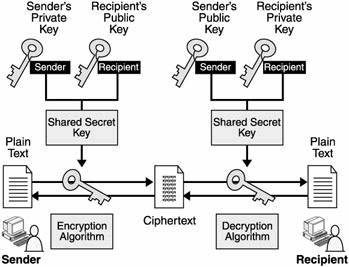
\includegraphics[width=0.65\linewidth]{../3.jpg}
\end{figure}
\end{center}
\end{frame}
\subsection{Giao thức Diffe-Hellman}
\begin{frame}{Diffe-Hellman}
\begin{center}
\begin{figure}
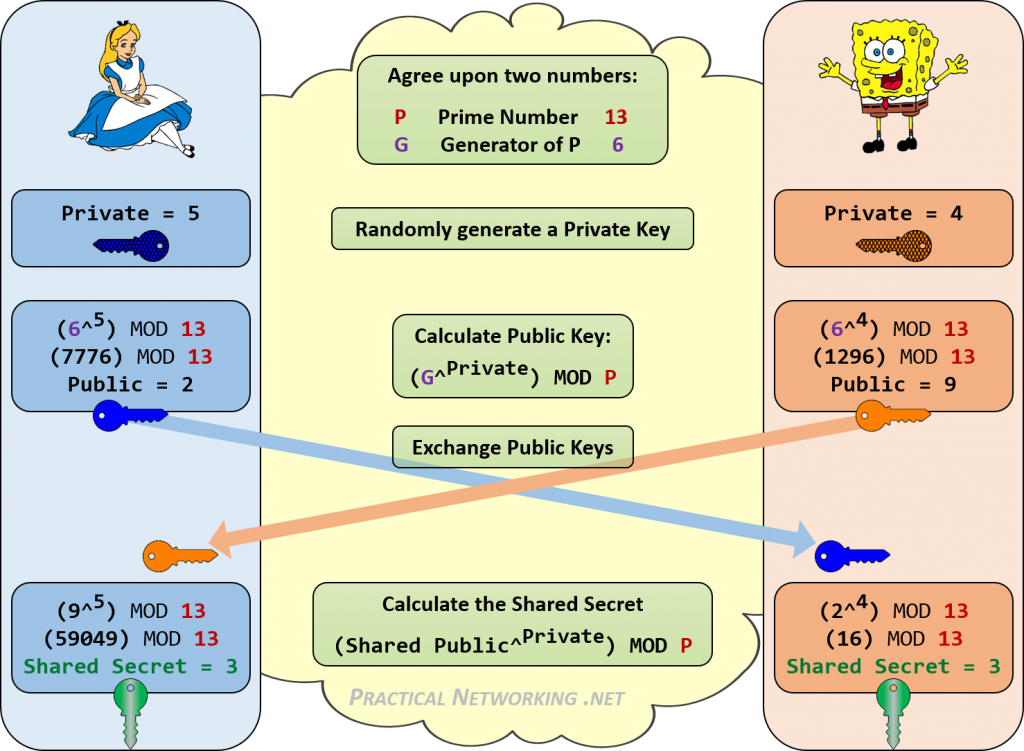
\includegraphics[width=0.9\linewidth]{../diffe-hellman.png}
\end{figure}
\end{center}
\end{frame}
\section{Đường cong elliptic}
\begin{frame}{Định nghĩa}
Một đường cong elliptic curve được xác định bởi phương trình đường cong
\begin{itemize}
\item \textbf{phương trình dạng Weierstrass}
\begin{displaymath}
E: y^2 = x^3 + Ax + B
\end{displaymath}
với điều kiện $A, B \in \mathbb{F}$ thỏa mãn $4A^3 + 27B^2 \neq 0$.
\item \textbf{phương trình dạng Montgomery}
\begin{displaymath}
M_{A,B}: By^2 = x^3 + Ax^2 + x 
\end{displaymath}
với điều kiện $A \in \mathbb{F} \setminus \{-2, 2\}, B 	\in \mathbb{F} \setminus \{0\}$ và $B(A^2 - 4) \neq 0$ 
\end{itemize}
\end{frame}
\begin{frame}{Elliptic trên trường }

\end{frame}
\section{Chứng thư số ẩn}
\section{Cài đặt}
\end{document}